\documentclass{article} % For LaTeX2e
\usepackage{nips14submit_e,times}
\usepackage{hyperref}
\usepackage{url}
\usepackage{listings}
\usepackage{color}
\usepackage{graphicx}
\title{A Comparison of Online learning Na\"ive Bayes Classifiers on RSS Feeds using Apache Spark}


\author{
Ahmet Anil Pala\\
\texttt{aanilpala@mailbox.tu-berlin.de} \\
\And
Franziska Adler \\
\texttt{minza@mailbox.tu-berlin.de} \\
}

\newcommand{\fix}{\marginpar{FIX}}
\newcommand{\new}{\marginpar{NEW}}

\nipsfinalcopy % Uncomment for camera-ready version
\renewcommand\paragraph{\@startsection{paragraph}{4}{\z@}%
            {-2.5ex\@plus -1ex \@minus -.25ex}%
            {1.25ex \@plus .25ex}%
            {\normalfont\normalsize\bfseries}}
\makeatother
\setcounter{secnumdepth}{4} % how many sectioning levels to assign numbers to
%\setcounter{tocdepth}{4}    % how many sectioning levels to show in ToC
\begin{document}


\maketitle

\begin{abstract}
In Text Classification Na\"ive Bayes Classifiers are popular due to their simplicity and find application in the field of spam email detection and discovery of specified web content \cite[p. 225]{ertel2008}. For instance, in order to predict a category like spam or ham for an email. A probabilistic classifier like Na\"ive Bayes can come in handy assuming that the data distribution is static over time, all data is always accessible and query time does not play a major role. For adapting real world problems and their dynamics this might not be sufficient. For applications requiring immediate processing of new data and answering queries in real-time, instead of traditional learning approaches, more real-time-ready learning techniques involving sophisticated model updates have to be devised. The reason why model updates are necessary is the prevalence of shifts in the statistical distribution of the target classes in online-learning scenarios. This is called \textit{concept drift}. Also aspects of scalability should be considered since concept drifts are common in situations of large data quantities arriving via streams with high data rates \cite[p. 4]{tsymbal2004}   

In this project we use RSS feeds from various news agencies for classification on a distributed system. The focus is on the evaluation of several Na\"ive Bayes classifiers which implement the online learning paradigm by using different model update techniques.  The evaluation concentrates on the handling of concept drifts. First part of this report explores the theoretical foundations of the relevant concepts as well as the explanations of the conceptual challenges we face and the methodology we follow for implementation and the evaluation. The second part digs in more details of our implementation such as how the different classifier approaches are realised. Furthermore the evaluation of their performances are analysed and presented.

\end{abstract}

\section{Theoretical background}

\subsection{Na\"ive Bayes classifier}
As mentioned Na\"ive Bayes classifiers are probabilistic classifiers which are simple but effective in text classification. They operate on the basis of the Bayes Theorem and assume independence of features. Here the feature values are normalised words frequencies occurring in a document. The probability of a word $w_i$ belonging to class $y \in Y$ is given by $P(y|w_i)$ and can be reformulated with Bayes Theorem to its conditional probability and a priori probability $ P(y)$ of class $y$. Both can be derived from frequencies of documents and words.
$$
P(y|w_i) \propto P(y)P(w_i|y)
$$
The computation of the joint probability over a documents features will give the probability for a  document $d$ belonging to a certain class $y$. Instead of multiplication the logarithm is used to avoid underflow by multiplying with zero:
$$
P(y|d) \propto P(y)\prod_i P(w_i|y)\space
\textrm{,  bzw.:    }
P(y|d) \propto log P(y) log \sum_i P(w_i|y),
$$
Applying for all classes will give the decision rule which categorise a new text document according to its most likely class which is the one with the highest joint probability value.
$$
\arg\max_y\{ log P(y) log \sum_i P(w_i|y)\}
$$

\subsection{Challanges/ Concepts}

\subsubsection{Concept Drift}
Most online learning scenarios including ours, news feed mining, is susceptible to the phenomenon called $concept$ $drift$. Concept drift occurs when the statistical properties of the target variable to be predicted change over time. Concept drift can manifest itself in different ways as explained in \cite[p. 1]{KunchevaEnsembleOverview08} . Firstly, shifts in the prior class probabilities or class-conditional probabilities could be the indicator of a concept drift. Likewise, if the relevance between a certain set of attribute values, clues, and certain class predictions change, this could signal a concept drift. Moreover, abrupt increase in the model complexity can be a sign of the concept drift as well for the applicable predictive models. Finally and most importantly, prediction accuracy serves as the most widely-used criterion for detecting the presence of a concept drift. 

The sources of the concept drifts are diverse depending on the application. For example, in spam filtering applications, user changing his/her mind about what is spam and what is not is an example of a concept drift \cite[p.8]{Gama2014}. In our classification scenario, news feed items categorisation, concept drifts can directly stem from the shift in the media attention which is naturally drawn to the emerging real-life events and its implications on the set of vocabulary news writers use to explain emerging phenomena. For example, a new music album titled  "Anarchy in the UK"  is introduced and sold millions of copies in short time hence became the topic of many news articles. Since the terms in the title suggests that the chances are that this item could be linked to the category 'politics', most probably the naive bayesian classifier will capture the statistical correspondence of these words to its corresponding what-it-would-be-categorized-as-in-past category and lead to false predictions.

Different ways of handling concept drifts proposed in literature are outlined and briefly explained in \cite[p. 1]{KunchevaEnsembleOverview08}. These different approaches can be classified according to 4 different criteria. First criterium is whether instance-based or batch-based processing of the stream items are employed. Since, instance-based processing is mostly too costly in terms of CPU load, batch-based processing where the continuous stream is discretised as batches are mostly used. Secondly, concept drift handling differs by the mechanism of the drift detection. There are two common kinds of concept drifts detection mechanism namely explicit detection and implicit-detection. Explicit-detection mechanism takes a detection action upon the detection such as retraining the model based on the recent items. On the other hand, implicit-detection only continuously adjusts the weights of different classification parameters as a function of concept drift indicators such as error rate, accuracy, etc. These parameters could be the weights of the members of the ensemble classifiers letting the models trained with the obsolete data fade. Moreover, another criterium for the above-mentioned classification is whether classifier-specific or classifier-free action mechanism is employed. In the former, the detection and action mechanism depends on the nature of the classifier and cannot be applied to the all kinds of classifiers. In the latter, the detection is bound to the accuracy and the action is updating the training data so it works with any classifier. Finally, concept drifts can be handled by a single classifier or an ensemble of them. When an ensemble is employed, the prediction decision is jointly taken by a dynamic combiner logic that forgets some of the classifiers which performs bad. Furthermore, although the drift detection action is usually implicit in the ensembles, every now and then ensemble can drop a member by running the \textit{replace the loser} policy \cite[p 18]{kolter}.

For this project, we use three different stream learning approaches. They all do batch-based processing using a single classifier for explicit concept drift detection. In terms of classifier-dependency of the concept-drift handling methods, two of them implement classifier-free methods for detection and taking action for the drifting concepts and one of them employs classifier-specific approach. Details regarding these different stream learning approaches we use are discussed in the Methods subsection.


\subsubsection{Streaming}
In order to deal with the continuous nature of the data, traditional programming primitives are not of much help and mostly distracting. In order to make programmers job easier, libraries providing higher level abstractions for stream data are introduced. These libraries usually discretise the continuous input stream into batches and give the programmer a local view of the stream allowing him/her to grab only the data from one batch at a time. Hence, programmer writes code to handle one batch of the discretised stream and the streaming library run this piece of code on all the batches sequentially as they arrive. For instance, programmer wants to use a flatmap function and he writes only one line of code where the flatmap function is called and the streaming library executes this line many times for each arriving batch as if in a loop. This abstraction takes care of all the chore of updating the data structures storing batch elements and bookkeeping loop variables to implement repetitive execution logic, letting the programmer concentrate only on the streaming logic of the application. 

\subsubsection{Distributed Systems}
With the Internet, data availability seems not to constitute a problem anymore. Aspects of storing, processing and mining those data amounts were reconsidered in the past years and led to the raise of new technologies. A single CPU can not accomplish the processing of those data quantities, especially if the algorithms are computationally intensive like most of the prediction algorithms from the field of Machine Learning which are widely used in data mining. To handle it, the parallel execution of computation is spread over a cluster of machines with an underlying system responsible for scheduling, load balance and fault tolerance is proposed \cite[p. 10]{zaharia2010} . The forerunner of this cluster model was Hadoop, now several frameworks which extend this work are developed and allow wider functionality and significant performance improvements. Even though these frameworks are centered around data processing and they provide nice abstractions such as MapReduce for ease of use, software developers need to be aware of the distributed nature of such systems and parallel execution models. This might be clear to those coming from a Distributed Systems background but challenging for data engineers or developers related to data mining who are more used to sequential arrangement of data processing. 

\subsection{Methodology}
As mentioned previously in the report, the major aim of the project is to compare different model update techniques implemented as the variants of the same Naive Bayesian Classifier in terms of their capability in adapting/capturing concept drifts. For this purpose, we evaluate one offline (as baseline) and three online classifiers.

\subsubsection{Offline Learning}
Offline learning assumes the access to all training points at once. From this initial training set the model is constructed to classify new data instances. This means after the training phase the learning is finished and in case of Na\"ive Bayes  the conditional probabilities which are the basis for the decision rule are fixed. The number of training items is hardcoded as the training phase takes place once and there is not much room for sophisticated dynamic variables for the parameters of the predictive model.

\subsubsection{Online Learning}
We consider three different online learning approaches two of which are slight variations of each other and both implement explicit-detection of concept drifts. As for, the third one, it is considerably different and it features implicit-detection methods for concept drifts. However, all three have a set of  features in common. To be more specific, they all are single-classifier approaches and all utilise a \textit{sliding window} of recent data points to be used for the potential updates of the predictive model. What first two approaches differ is the way predictive model updates are triggered. The first approach, called the bruteforce update, rebuilds the model at fixed intervals by using the data items stored in the sliding window.\cite[p. 24]{streamingSlides} The second variation called, error-triggered updates, waits for the accuracy rate to go below a certain threshold which is hardcoded. Third model, called incremental updates, implements a different model update scheme than first two. Instead of rebuilding the model with the recent data, it incorporates the recent data coming from the last window into the model. While doing so, it scales the feature vectors of the recent data by the learning rate and the past data by learning rate subtracted by one. Learning rate simply specifies the amount of adaptation to the recent items to be done and the amount of 'forgetting' of the past models. Use of a dynamic learning rate is elevated by increasing rates of error. This enables the incremental updates approach to 'silently' detect concept drifts and take the recent data into more consideration than the past by scaling down the feature vectors of the past models and taking the feature-vectors of the recent items almost as they are. One crucial point worth mentioning about incremental-updates model, it continues the training of the classifier with every incoming batch of data no matter what the learning rate is at the moment. This makes the training and test set simply perfectly overlap onto each other. In other words, every incoming item is used for updating the model after the prediction is done and the immediate feedback on the outcome of the prediction is used for tweaking the learning rate. 

\section{Empirics}
\subsection{Data}
%write here
Data we are using are RSS (Really simple syndication) items streamed from RSS providers of news portals such as BBC, CNN, CNET and Washington Post. An RSS Item is combination of some tags describing the content of the feed item and some meta-data about it such as publication date, url, etc. in XML structure. An example RSS item is given below.

\lstset{
    language=xml,
    tabsize=3,
    %frame=lines,
    caption=An Example RSS Item,
    label=code:sample,
    frame=shadowbox,
    rulesepcolor=\color{gray},
    xleftmargin=20pt,
    framexleftmargin=15pt,
    keywordstyle=\color{blue}\bf,
    commentstyle=\color{OliveGreen},
    stringstyle=\color{black},
    numbers=none,
    numberstyle=\tiny,
    numbersep=5pt,
    breaklines=true,
    showstringspaces=false,
    basicstyle=\footnotesize,
    emph={food,name,price},emphstyle={\color{magenta}}}
    \lstinputlisting{sample_feeditem.xml}.

Here, we are only interested in what is in the publication date, description and title tags. Publication date is crucial for computing interval-based prediction accuracy metrics and in-batch ordering. Description and title constitute the document we want to categorise in our case as we want to mine RSS feed items as opposed to mining the news articles themselves. Therefore, there is no need for fetching the actual article for the full text. The URLs where we draw the RSS items are from different RSS provider defines the category of the RSS items to be streamed since RSS providers provides different URLs for streaming RSS for different categories. We stream from 13 different RSS URLs for 5 different categories namely business, politics, tech, health and entertainment. These serve as labels of the RSS items and also what is to be predicted. URLs we use can be found in the urls.txt file under the resources folder.

One difficulty of working with data streams is the volatility of the data hence it inherently requires real-time data processing. In other words,  data should be handled as soon as it arrives. Since it is only possible to process data after implementing the text classifier and get it running, there was no straightforward way of utilising the data streamed during the development of the project. As Data scarcity evidently would pose a serious problem for a text classifier especially considering that we aim to detect concept drifts, we were compelled to find a way to facilitate the data being streamed while developing the application. To this end, we decided to first archive the stream data, then broadcast/stream this data through one of the local ports on the development environment and finally let the streaming application consume this archived data broadcasted data once the development is complete. This way, we could take the time needed for the development and meanwhile did not lose any data since the very first day we conceived the idea of mining news feeds items for this project.
\subsection{Software}
%write here
For realising the stated approaches we are using Apache Spark and MLlib. Apache Spark is an open source processing engine for parallel processing of large scale data. Spark works on top of a distributed storage and uses a cluster manager cluster manager like Yarn or Mesos. For the purpose of this project the locale storage was used as simulated distributed storage which is integrated in Spark for developing and testing reasons.  \\
While the Spark core handles scheduling and load balancing, on top of it, supplementary modules provide additional functionality for streaming, Machine Learning  algorithms and graph computation. The main programming abstraction in Spark is called RDD (resilient distributed dataset), a collection of objects partitioned across different machines for parallel programming. Besides map and reduce, some other parallel operations on RDDs like filter, collect and foreach etc. are provided. For shared variables broadcast variables and  accumulators can be used.

\subsection{Implementation}
%write here

Our implementation effort can be broken in two main parts namely initial streaming and the implementation of the stream learning algorithms.

\subsubsection{Initial streaming}

The starting point for the implementation was designing and implementing a \textit{hook} for stream data. Usually, it is trivial to feed Spark Streaming with a stream but in our case we had to be careful with the amount of data that we can process for the observations in the limited timeframe would be left after completing the implementation  specially considering that we aim to detect concept drifts, we were compelled to find a way to facilitate the data being streamed while developing the application. To this end, we decided to first archive the stream data, then stream this data for the second time through one of the local ports on the development environment and finally let the streaming application consume this manually streamed data once the development is complete. This way, we could take the time needed for the development and meanwhile did not lose any data since the very first day we conceived the idea of mining news feeds items for this project. Below diagram describes how this initial handling of the data is realised. 

In the figure, Spark Streaming discretises the incoming stream by breaking the data into batches to be processed in first in first out order. We simply run this flow which also does after doing in-batch ordering of items according to their timestamps to accumulate a txt file for the RSS archive to be streamed later. Additionally, this streaming also creates a dictionary, everytime it runs inserts new vocabulary into the dictionary along with their associated hashcode which serves as the unique identifiers for the terms. In the source code, implementation of the Initial Streaming tasks can be found in \textit{rss.categorizer.util} package, RSS Fetcher.java and FeedRefiner in particular.
\begin{figure}[htbp]
  \centering
  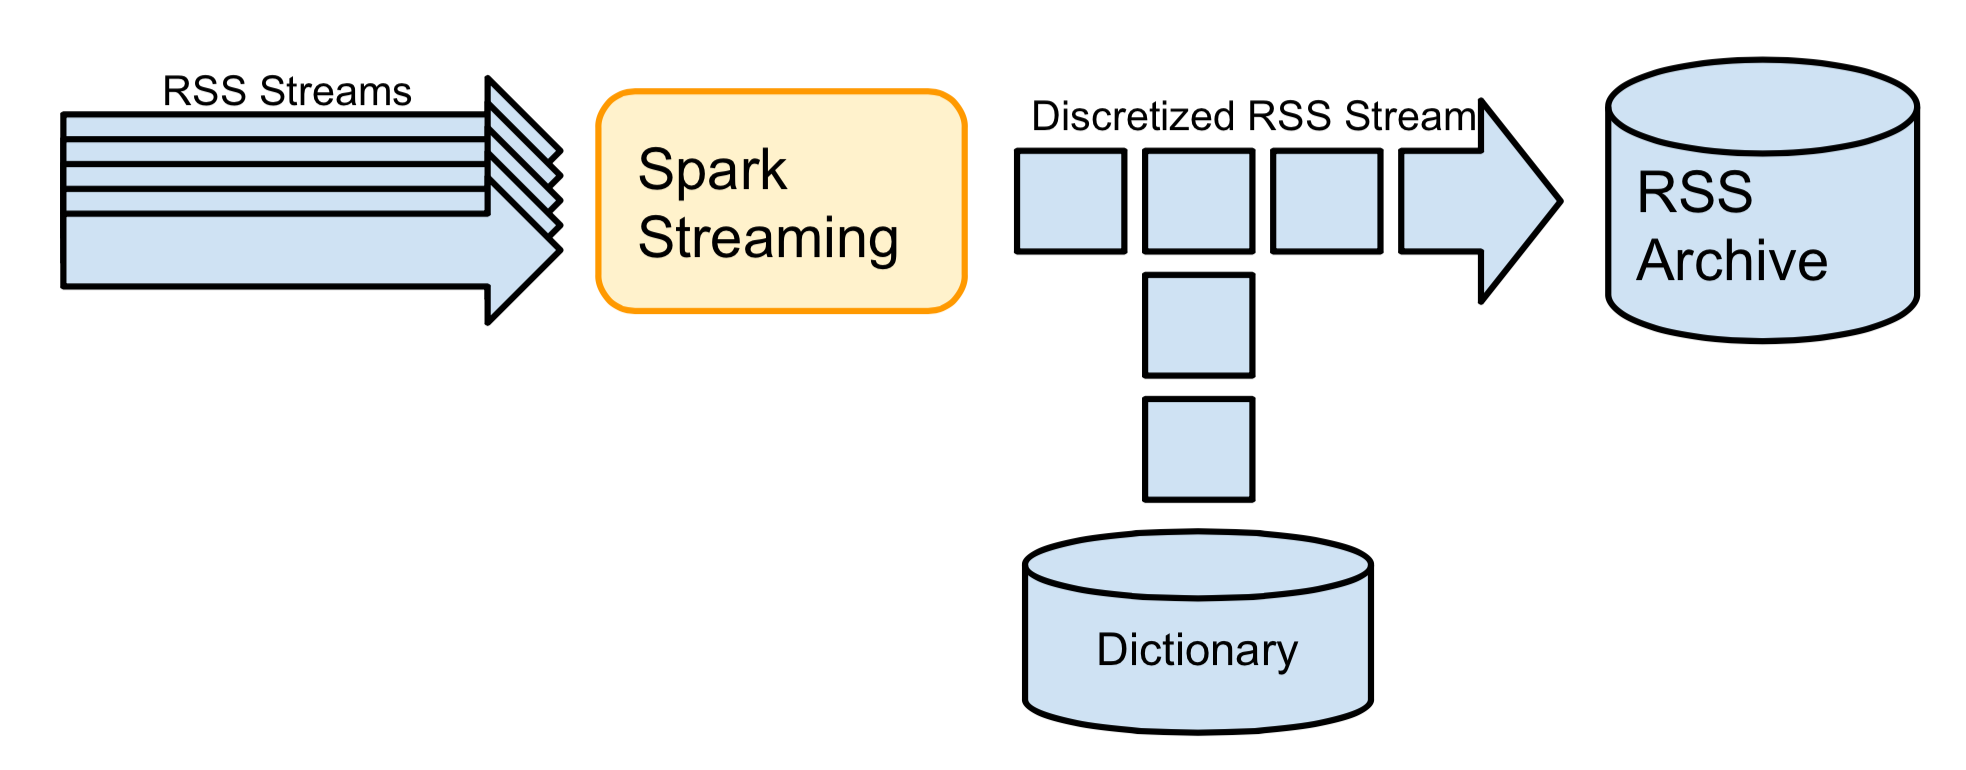
\includegraphics[scale=0.28]{./figures/initial_streaming.png}
  \caption{Initial streaming}
\end{figure}


\subsubsection{Stream Learning Algorithms}

For the implementation of the stream learning algorithms as the core of our feed categorised application, we first attempted to use Spark Streaming and NaiveBayesian classifier provided by Spark MLlib in combination to facilitate convenient streaming abstractions of Spark Streaming library and also use the NaiveBayesian classifier which is a very flexible and customisable implementation of the algorithm and allows the use of different feature vectors other than term-frequency. This approach failed due to a very strict restrictions on shared state variables in Apache Spark. More specifically, in order to implement stream learning algorithms which does explicit-detection for conceptual drifts, some state variable needs to maintained which the control flow of the stream algorithm depends on. This means that there needs to be a globally shared state variable which is broadcasted whenever the state variables are updated. Apache Spark does not allow this to happen. For example, in the case of error-triggered update approach, there should be a boolean variable that becomes true whenever error rate, which can be maintained by means of an accumulator, goes below the threshold. A potential solution to this problem was to use the updateState function provided in Spark Streaming. Although this appears to be specifically designed for overcoming the difficulty of keeping state variables with the streaming abstraction which essentially treats every line of code as statements in a loop, this does not solve our problem with not being able to retain a single state variable. This is because, what updateState function offers is to join the current stream batch onto the past one and in this fashion build an incrementally accumulated and key-indexed RDDs which is not suitable model for storing a single-variable state. 
 
The workaround we found was having the driver program done the heavy lifting of the tasks of model building or model updating after collecting the RDD items partitioned across the nodes of the cluster by using the \textit{collect} function. This way, a state variable can be stored in the driver program and can be updated easily. However, this only does not fully solve the whole problem. This is because, the function \textit{collect}  can be only used for RDDs. However, with the streaming enabled, instead of RDDs, we only can get out hands on sequences of RDDs. After having tried hard to get this combination of three different libraries namely Spark Core, Spark Streaming and Spark MLlib and experienced the above mentioned technical difficulties which can be arguably caused by either the design choices of the libraries or the current incompatibilities between them, and also having considered that the main challenge of the project is supposed to be rather on the study of the relevant concepts and the experiments rather than a specific library, we decided to give up on using Spark Streaming and simulate the streaming behaviour by traditional programming primitives such as a plain loop which draws a batch of the labeled points in every iteration from a file.

All four variants of the learning algorithm has a similar structure. For the explicit-detection approaches what changes from one to another is the triggering logic of the model update procedure. Although the forth variant, the incremental updates, looks pretty different, when the details are abstracted away, it follows the same steps as the other ones. Therefore, these all four variants could be depicted in one general picture.
\begin{figure}[htbp]
  \centering
  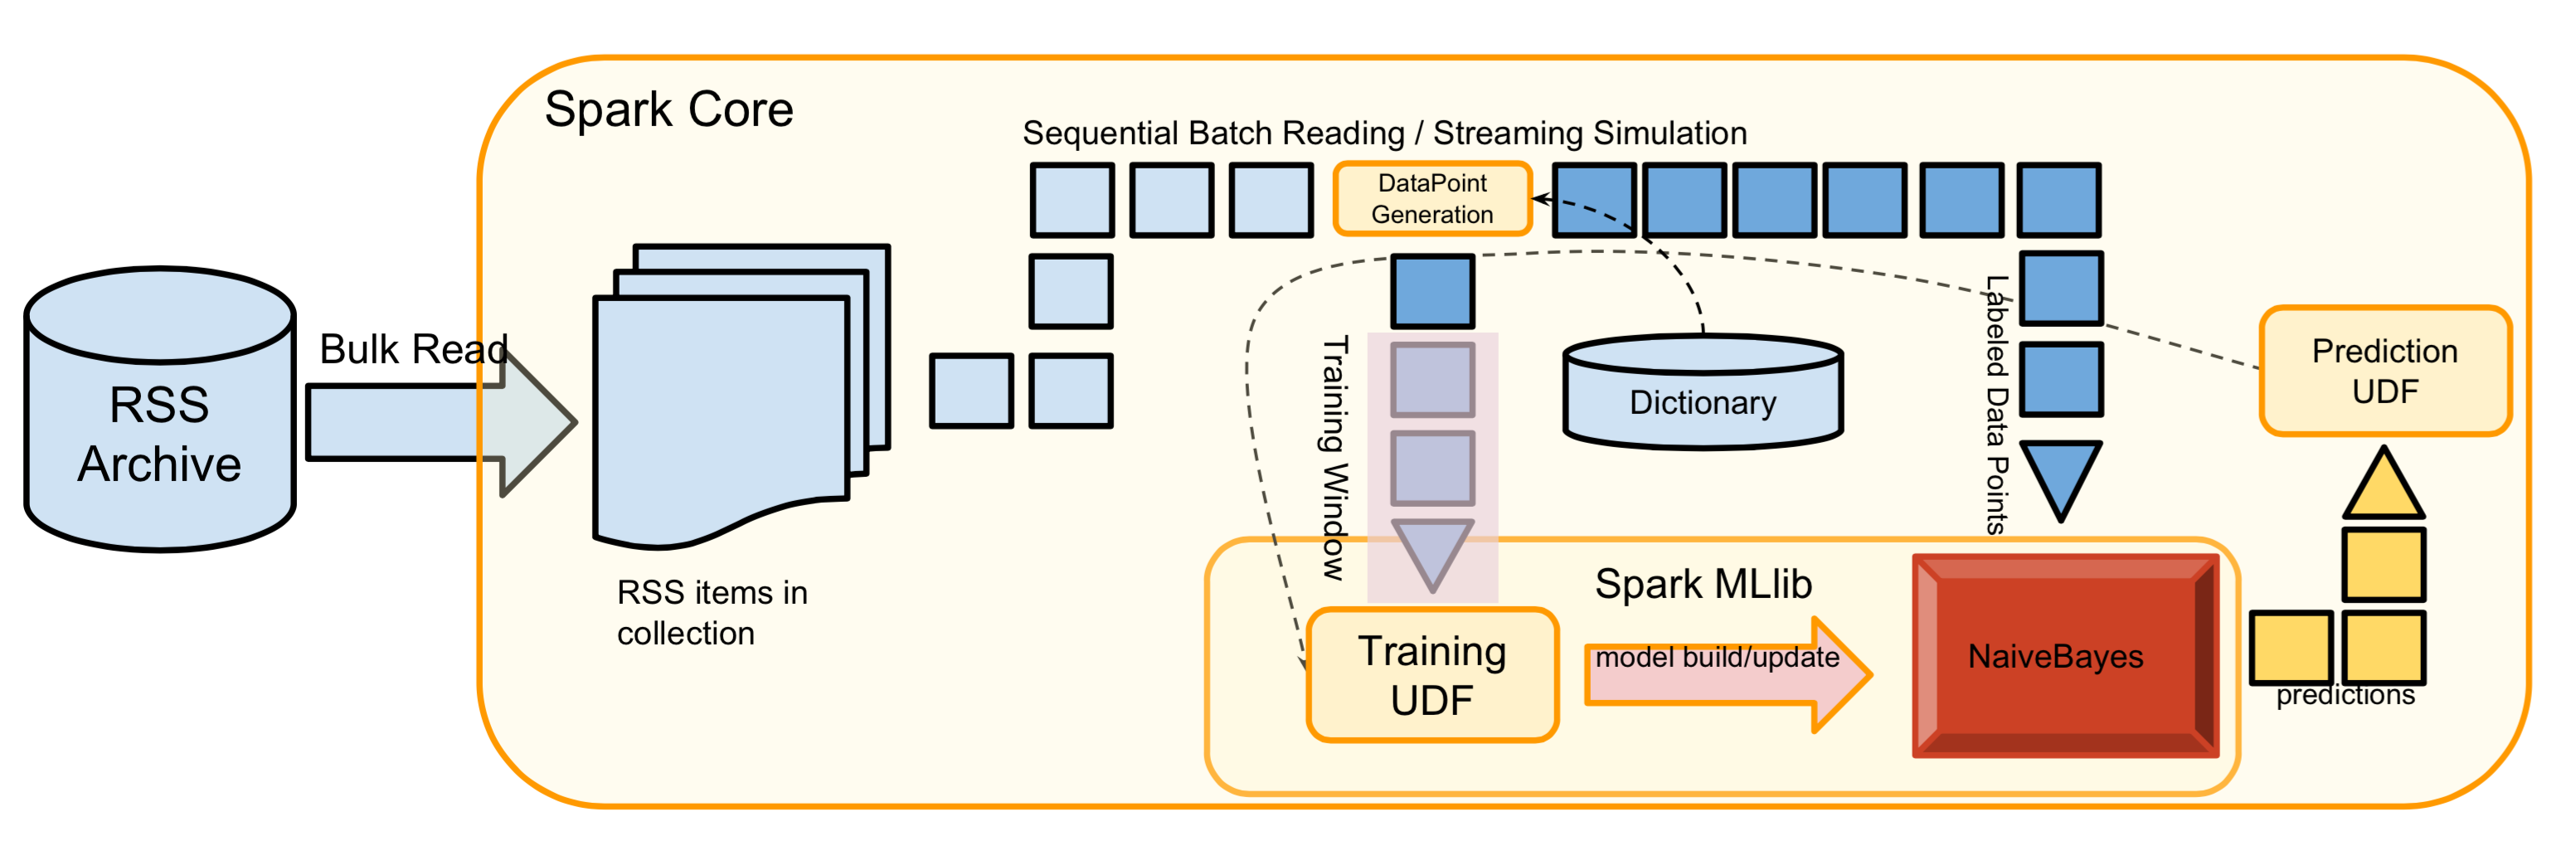
\includegraphics[scale=0.24]{./figures/streaming_diagram.png}
  \caption{Streaming diagram}
\end{figure}

In the figure, we see that RSS archive file which is streamed by the initial streamer application whose details are discussed in the previous section is read into a collection located at the driver program. And then, from this collection the RSS items are drawn in batches (one or multiple RSS items in one batch, a parameter) at every iteration of some loop that simulates the Streaming logic.

The batches here corresponds to the discretised batches in Spark Streaming. Then, for the training and prediction, in order to create data points, we have DataPointGeneration component. It converts feed items into labeled data points where label is the category of the individual RSS Item which is obtained by the hardcoded mapping of Feed URL and their corresponding variables of double type that represents individual topic categories. Additionally, at this stage, some preprocessing done on title and description of stream items. More specifically, symbols and non-ASCII characters are discarded and stop-words eliminated by using a simple hardcoded stop-word dictionary.  

Furthermore, the datapoint part of the labeled datapoint consists of a sparse vector of features indices and feature values which are both represented as an array. Feature indices are simply obtained from the dictionary which is basically a mapping between the dictionary term to their corresponding hashcode. For each term occurring in the title or the description of the feed item, its corresponding hashcode is fetched from the dictionary. As for the feature values, term-frequency of the terms are used assuming feed items title and description constitute a document . 

Then we have a \textit{TrainingUDF} which is pictured as black box in this abstract picture as this is the component where different variants of stream learners differ from each other. First three variant maintains a sliding window of a number of batches where this number is a parameter. Whenever a training is triggered, the training data in this sliding window is used. In the forth variant, incremental updates, this sliding window always contains the most recent batch. 

It is worth mentioning that, this training UDF is only triggered by some state variables which are controlled by a logic which is different for every variant. So, when it is fired, the part of the collection of RSS Items whose indices falls within the sliding windows indices are paralleled via the \textit{parallelise} call provided by Spark Core and then used for model training or model update purposes whose details again up to the model update variant that is used. After the parallelisation of the training dataset, parallelised RDDs can be passed to the MLlib's Naive Bayesian model building functions for training. After the data point generation, the initial training is the same for every variant. However, after the initial model is created, when the \textit{TrainingUDF} is fired again, all the variants except for the the incremental model trivially retrains the model based on the data in the training window. As for the incremental model, it updates the model by incorporating the recent items  from the training window into the bayesian model. 

However, instead of using the term-frequency for feature values, the forth variant uses TF multiplied by the learning rate for the new training points and also overwrites the feature values of the vectors of the training data by multiplying by learning rate subtracted from 1. This way the Bayesian model is incrementally updated. In the case, the \textit{TrainingUDF} is not fired, it just does not do any training although it still updates its training window as more items arrive. Following the other branch from the data generation point, for every data point the prediction method provided by the Naive Bayes model object is called and predictions are obtained. Then, there is \textit{PredictionUDF} that calculates the cumulative accuracy rate as it receives the predictions and labels by simply checking for equality. Moreover, \textit{PredictionUDF} manages a very crucial task: it dynamically controls all the state variables which are used for triggering of \textit{TrainingUDF} and changing the learning rate for the incremental updates variant.

\subsection{State Variables}
Each variant has a different implementation of \textit{TrainingUDF} triggering functionality and it is controlled by a boolean state variable. In the batch model, there is no need for training after the initial training, hence there is no triggering of \textit{TrainingUDF}. 
In the case of bruteforce update variant, \textit{PredictionUDF} fires the \textit{TrainingUDF} at the fixed intervals which is a parameter for the stream learner implementation. For the error-triggered updates variant, \textit{PredictionUDF} fires the \textit{TrainingUDF} whenever the cumulative accuracy it computes goes below a threshold which is again a parameter that can be tuned by hand. As for the incremental updates model, there is again no need for triggering of the training in the incremental updates model since \textit{TrainingUDF} of it is always on, it always updates the Naive Bayes Model. This is a direct implication of the implicit concept drift detection behaviour of this variant.

Learning rate variable is used only for the incremental updates variant. For this, we designed a function that converges to 0 as the prediction accuracy improves and to 1 as it decreases. So, after every batch, we know the change in the cumulative accuracy and if there is an increase in the overall accuracy, we increase the current domain index of the learning rate function by a step size(a parameter) and read the range value which is the learning rate itself. The functions range interval is the [0,1] and domain interval is the Java representation of all positive rational numbers. The function is depicted below for the domain interval [0,50]

\begin{figure}[htbp]
  \centering
  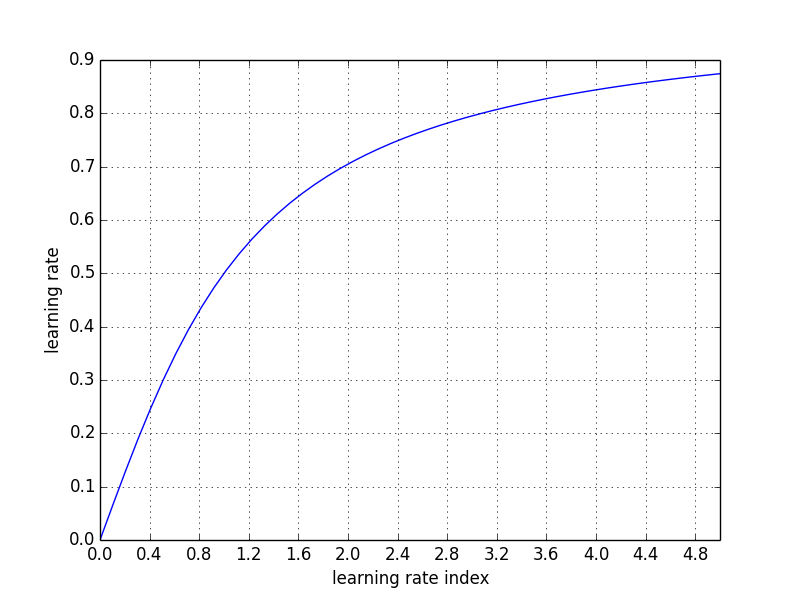
\includegraphics[scale=0.54]{./figures/learning_rate_function.png}
  \caption{Learning Rate Function}
\end{figure}

Full implementation of stream learning algorithms can be found in the \textit{rss.categorizer.classifier} package of the attached source archive. Additionally, our failed attempts to get Spark Streaming together with Spark MLlib working can be found in \textit{ rss.categorizer.stream}. All the sources can be also accessed through the repository at \url{https://github.com/minziska/AIM3_project}

\subsection{Evaluation Setup}


\subsubsection*{Evaluation Measure}

To detect concept drift different error measures like expected error rate - or in case of dealing with ensemble classifiers - error decomposition can be used to observe changes in the probabilities which might relate to concept drift.\cite{Gao07ageneral}  Since we are using MLlib and it is hard to reach the inner properties of the computed model to compute elaborate measures we took cumulative accuracy as a very simple evaluation measure.  Accuracy is the  proportion of correctly predicted labels among all predictions. For the evaluation, we successively computed the accuracy with every new incoming data point to calculate the cumulative accuracy over all data points and also the cumulative accuracy per testing interval.

Before any evaluation, we intuitively expected the accuracies of window-based techniques to be higher than the batch model. Additionally, retraining is expected to adapt to concept drift which we hope to detect by comparison of batch model with the different model update techniques. Also the incremental model is expected to outperform all others.

\subsubsection*{Offline classifier}
In three weeks we received 3659 data points from the streams. This rather small amount of data restricted us to choose a small training set size. And, in order to set a fair base for later comparison between models, for each different stream learner variant, we fixed the initial training data at 600 data instances which equates to the first three days of streaming news feeds. 

Our first approach, the offline variant, is used as a reference model. After the training phase, we have chosen three disjoint test sets with 1000 data points each as seen in the block diagram below to monitor possible performance changes over time. Our size of training and test set differ from traditional offline learning test setups which usually take a 50:50 to 80:20 ratio for set sizes. Obviously, the classifier performs better the more training data is available, but since we are also experimenting with sliding window approaches for the online classification which require a number of repetitions of training and testing intervals to monitor accuracy changes that is the basis for the detection of concept drifts in our experiments, we opted for this unusual 20:80 split. Due to this experimental setup, we are not expecting a very high performance accuracy in general but to detect changes in performance which could indicate some sort of concept drift.

\begin{figure}[htbp]
  \centering
  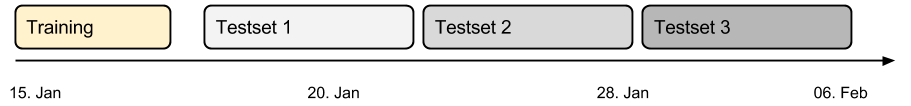
\includegraphics[scale=0.28]{./time_models/OfflineModel.png}
  \caption{Offline setup}
\end{figure}
\subsubsection*{Bruteforce}
As mentioned the second approach - the bruteforce method -  takes a sliding window of 600 data instances. We applied retraining phase three times and after every training a test phase followed to measure the performance of the previous training.  The test sets in this scenario are the same sets as used in the offline classification and contain 1000 data points. Except the last test set which will not be taken into further consideration because of its small size.

\begin{figure}[htbp]
  \centering
  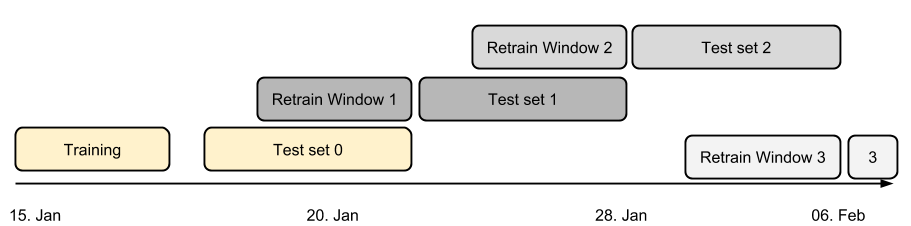
\includegraphics[scale=0.28]{./time_models/BruteforceModel.png}
  \caption{Bruteforce setup}
\end{figure}
\subsubsection*{Error-triggered}
As a variation of the bruteforce model with a fixed retraining interval, we used a threshold triggered retraining variant which will rebuild the model out of the sliding window as soon as the accuracy of the model goes below a certain threshold. The window size of the error-triggered model consists as well of 600 data points like in the previous models. We set the accuracy threshold to 63\% which seemed to be a reasonable choice due to our observations with the offline method. A sanity window of test points ensures that at least 300 new data points arrive before prematurely throwing out the rebuilt model. That means after every training at least 300 data points will be used to compute the performance and compare it to the threshold before the decision for retraining or not is made. Experimenting with smaller sanity windows lead to constant rebuilding due to the low accuracies of the undertrained models.  On the other hand, a longer sanity window inactivates the triggering behaviour of the model and make it rather like bruteforce model. With the chosen sanity window rebuilding is executed six times.

\begin{figure}[htbp]
  \centering
  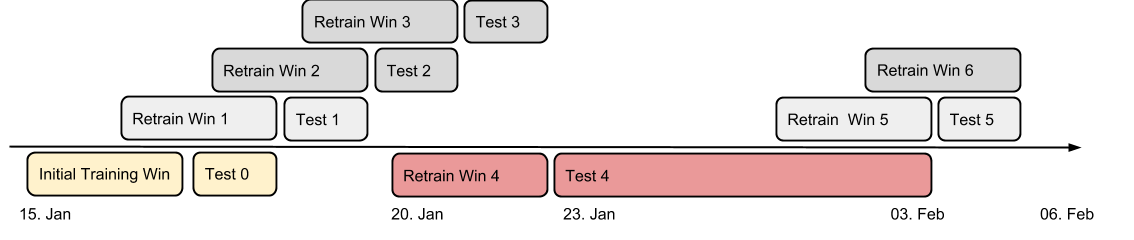
\includegraphics[scale=0.25]{./time_models/Errortriggered.png}
  \caption{Error-triggered setup}
\end{figure}
\subsubsection*{Incremental}
In the incremental model, unlike the other update models, following an initial training-only phase, all the incoming stream items are always used for training right after the prediction. So, this way the immediate information whether the prediction was good or bad can be used for improving the model on the fly. In other words, predictive model building and testing phases perfectly overlap in incremental model update method. We used this to achieve a real-time response to the changes in the data arguably making the text mining application more resilient to the conceptual drifts. The initial training size of 600 is used for this model update method as well.

\subsection{Evaluation results}

The overall cumulative accuracy of the offline classifier is around 60\% as visualised as a yellow line in the graph below. The result is plausible since we did not deal with bias or variance and therefore weight the features nor preprocessed the data like using a stemmer. The per interval cumulative accuracy is shown alternating in green and blue. The first oscillations of the interval accuracies can not be taken into account which are approximately the first 250 - 300 test items since cumulative accuracy needs at least some prediction values to be reliable. As explained before the prediction model was computed once in the the first three days of receiving data points and applied to four disjoint test sets which were received in a later point of time. The training items are not included in the graph, it starts with the first test point:
\begin{figure}[htbp]
  \centering
  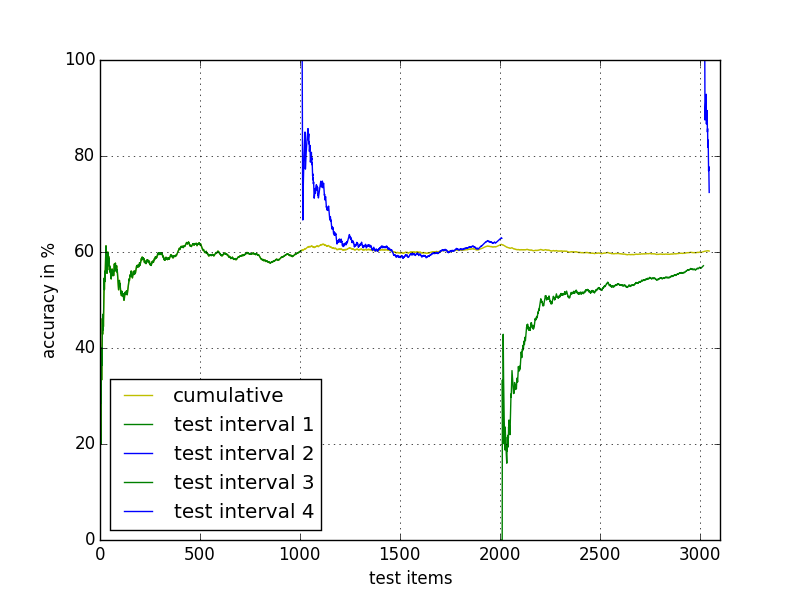
\includegraphics[scale=0.5]{./plots/batchPlot.png}
  \caption{Performance of offline learning with received test items over time}
\end{figure}

While the first two intervals do not differ much the third interval shows a worse performance. This means the model which was computed in the beginning of our streaming does not fit very good to test items in a two weeks later point of time and  might indicate some sort of concept drift.

The results for the bruteforce version which has the same testing setup but retrains the model after each test phase are shown in figure 8 and 9. The first test set will give the same results as the offline learning since they are both computed in the same way and the first retraining phase takes place after 1000 new instances arrived.The overall accuracies differ from the offline version by a notch. The graph shows nearly 63\% to 64\% of overall accuracy after the first retraining.
\newpage
\begin{figure}[htbp]
  \centering
  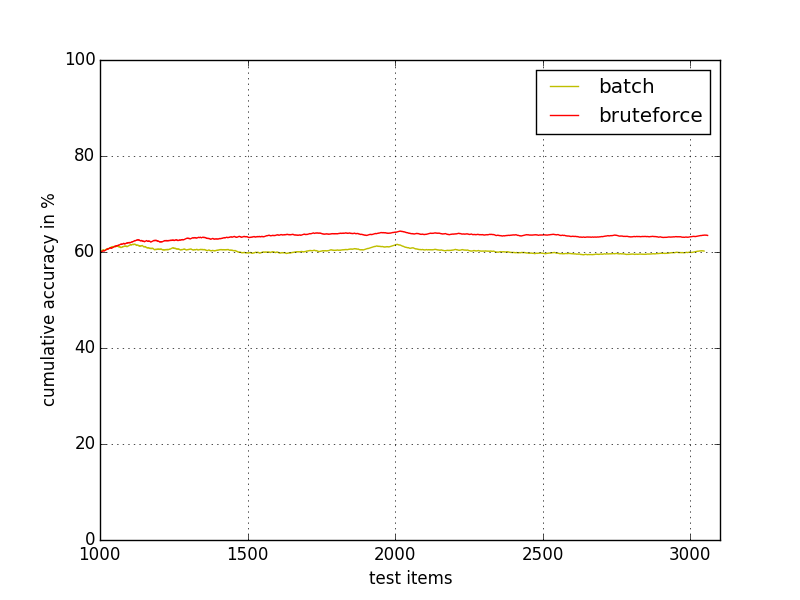
\includegraphics[scale=0.5]{./plots/overallBatchBruteforce.png}
  \caption{Overall accuracy for batch and bruteforce models after the first retraining}
\end{figure}

A one-to-one comparison of the different intervals of both models shows the following: The first retraining at data point 1000 improves the performance, the second retraining at test item 2000 does not perform as good as the first retraining on the following test set but is still better than the offline model. We assume that, this is a manifestation of a concept drift, but the interval size which is a parameter for the predictive model might not have been chosen well since the accuracy drops after the second retraining. The second retraining might have taken place to soon, while the first retraining seemed approximately right in time. Nevertheless we can say that the bruteforce method does perform better than the offline method.
\begin{figure}[htbp]
  \centering
  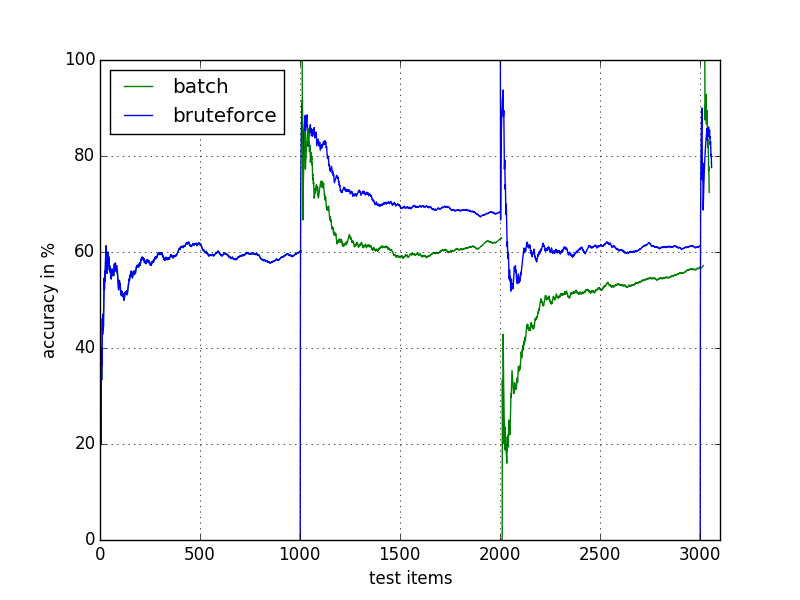
\includegraphics[scale=0.5]{./plots/bruteforce_batch.png}
  \caption{Per interval accuracy for offline and bruteforce method}
\end{figure}

The error-triggered model should handle this problem of fixed retraining phases and give us better estimation when retraining should be done. We used the accuracy of 63\% as the triggering threshold accuracy. Our choice of 63\% follows the heuristic that error-triggered model should not be outperformed by the brute force one in accuracy. Another parameter is the sanity window size. Accuracy points displayed in this graph are per-interval cumulative accuracies. It starts at 300 received test points which marks the delayed beginning of the first retraining of the error-triggered model due to its sanity window of 300 items.
 

\begin{figure}[htbp]
  \centering
  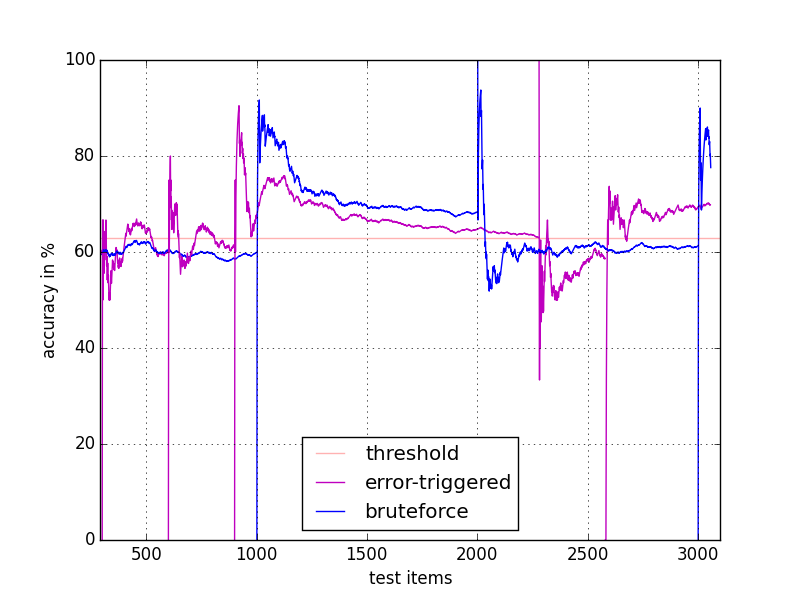
\includegraphics[scale=0.5]{./plots/errortriggered_bruteforce.png}
  \caption{Per interval accuracy for error-triggered and bruteforce method}
\end{figure}

As seen here the retraining in the error-triggered stream learner takes place two more times at test items 600 and 900 which are the multiples of the sanity window size. It follows by a stable model for over 1300 incoming test items and is retrained again two times. When interpreting these results, we should keep in mind that the test sets of the error-triggered models are much smaller than the bruteforce ones. However, the performance of the retrained error-triggered models are not necessarily much better than the bruteforce model except in the last interval starting at test items 2600. 

A stable error-triggered stream learner starts at test item 900, just 100 data points before the bruteforce retraining is done, but its accuracy decreases to the approximatly of the threshold shortly before 1000 test items point. With this drop, accuracy of the error-triggered model went below that of the brutforce model. This means that retraining the model at the 1000 test item point leads to a better prediction for a longer period as seen in the case of the bruteforce model. This might be caused by the conditional distributions before and after 1000 test items point are somewhat consistent and there was not any emerging/distribution changing items and a classifier which retrains itself at 1000 test point items will beat others. This rules out the possibility of an abrupt concept drift around 1000 test items point and onwards at least until 2000 test items point.  

As for incremental approach, results we obtained that it produces the best accuracy among other variants, going beyond 70\%. This is no surprise since its learning mechanism is totally different than periodic or non-periodic rebuilding approaches. Unlike them, the incremental approach never explicitly throws out the old training data and as a result of this possibility having an undertrained updated/retrained classifier is avoided unless learning rate goes to the upper extreme value of 1 which never happened. In our experiments, we tracked the change of learning rate as well as the cumulative accuracy. This is plotted in the graph below. 

\newpage
 \begin{figure}[htbp]
  \centering
  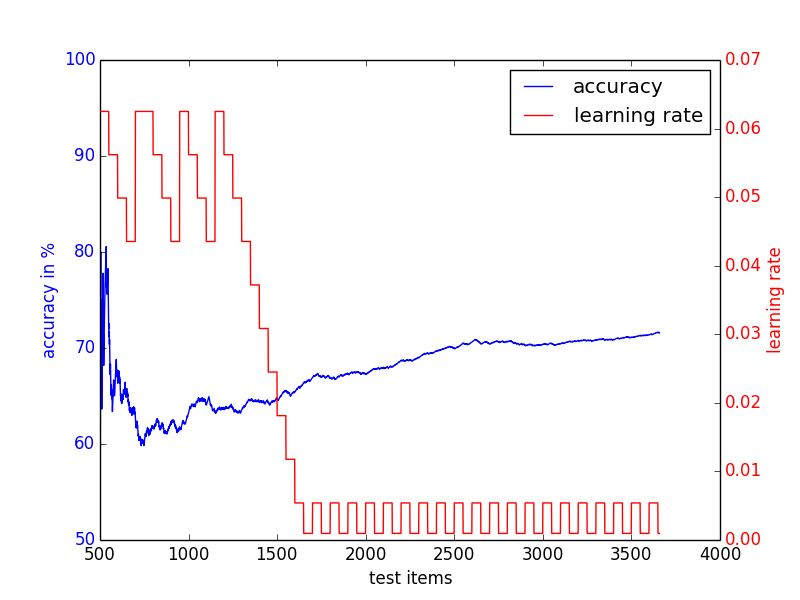
\includegraphics[scale=0.5]{./plots/incremental_plot.png}
  \caption{Incremental update model accuracy and learning rate change}
\end{figure}


We see that, initially both accuracy and learning rate fluctuate around 65 \% and 0.05 respectively. Then, accuracy starts to improve almost monotonically and meanwhile learning starts oscillating between 0 and 0.005   Three initial peaks that we observe in the learning function looks correlated with three times when accuracy sharply decreased. This is definitely an indicator of the times when the predictive model trained until the moment got somewhat less accurate than before and needs to be updated more aggressively by a higher learning rate. However, it is hard to say this might or might not be linked with a concept drift because except for the first drop in the accuracy all the rest is very minor and might be caused by some noise or outliers in the data.

 \begin{figure}[htbp]
  \centering
  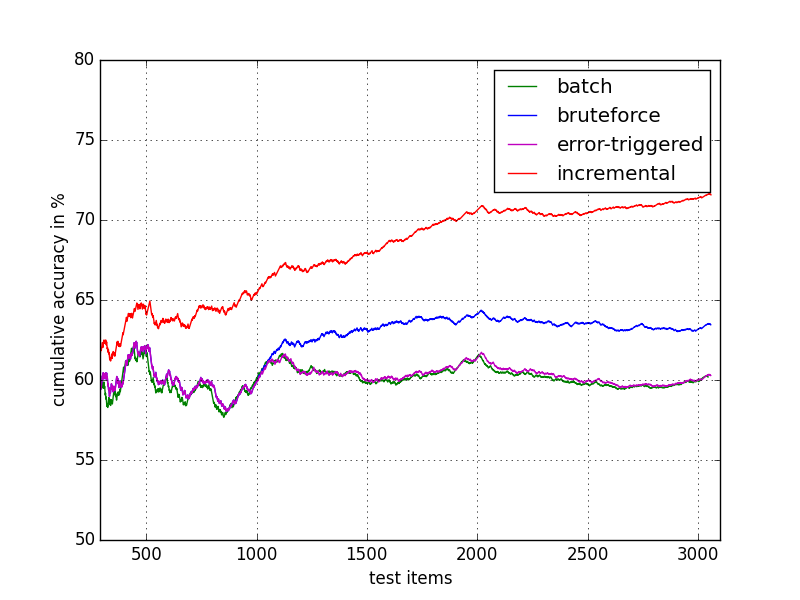
\includegraphics[scale=0.5]{./plots/allAcc.png}
  \caption{cumulative overall accuracies}
\end{figure}
The cumulative accuracies over all intervals in the figure above show that error-triggered and batch performance is nearly the same due to the oscillations the error-triggered models produce. It is obvious that retraining very often does not necessarily lead to better performance. In our case we had been lucky with choosing the intervals for bruteforce technique which reflects as well in the overall accuracy. There might be some sort of concept drift but this needs further exploration and more testing with different parameters and concept-drift detection methods.

\subsection{Conclusion}
In this project we tried to implement different online algorithms with a Na\"ive Bayes classifier to handle concept drift which we measured with simple cumulative accuracies. We planed to apply the classifier directly on stream data which encountered several technical problems due to the compatibility issues of different libraries we are using. After several changes a simulation of streaming and the implementation of the algorithms provided a basis for retrieving classification results for further evaluation.   

According to our assumptions concept drift might have been detected over the three weeks but with the given setup we can not identify which sort of concept drift nor when exactly. We did observe changes in accuracy performance of stream learners which are caused by either changes in the prior probabilities of the stream data or the changes in the conditional probabilities of Na\"ive Bayesian models if a retraining or update action is taken by the stream learner. These might or might not be linked to concept drifts. 
Moreover, we got to see the existence of myriad of possible parameters for stream learning algorithms which have to be very carefully chosen and tuned along the way. Specifically, initialising the state-variables as well as maintaining them are a crucial tasks and wrong choices there might lead weird behaviour such as no triggering or continuous triggering of the model update procedures. However, in order to inspect what selection of parameters are good, we simply need more experiment meaning more data. And in an online-learning scenario more data means more time, then someone could experiment with stream learners with different parameters. Data scarcity eventually proven to be a big issue in our case in both dimensions: data rate and data interval. Firstly, having observed that using 600 training items as the parameter choice for training window size is not enough to build mature classifiers resulting in undertrained classifiers and its consequences like retraining actions of stream learners having been rendered useless for handling of conceptual drifts that manifested itself as unsatisfactory accuracy values after retraining sessions, we wish to have hooked more RSS streams into our application which would increase the rate of the incoming data. Then, it would be possible to train classifiers without having to settle for too less data items while leaving enough days for testing, potential proper retrainings with more data points in training windows and monitoring of conceptual shifts. Secondly, if we could run the application longer, we would have more data to analyse and there would be more chances for real-life events to cause drifting-concepts in the stream data. This would allow us to  make more confident evaluations and draw more clear conclusions.







\bibliographystyle{unsrt}
\small{
\bibliography{literatureDB}
}
\end{document}
